\chapter{Characterization}

The goal of the work is to characterize the energy and latency of end-to-end Omni-directional(OD) Camera  systems both in the hardware and software pipeline and propose optimizations. As the existing OD camera systems are built from off the shelf camera devices and uses the conventional stitching algorithms, they capture, transfer redundant data and perform redundant computations. The redundancy can be attributed to the sptio-temporal correlation between the frames. The main challenge in OD panorama generation is to understand the data flow across the system and to make decisions on data abstractions needed at different subcomponents to reduce the total system power.

We characterize both monoscopic and ODS camera systems. The difference between them is the number of novel views needed is significantly higher for ODS compared to monoscopic. Both the systems at core use optical flow based stitching, so we will characterize generalized flow based stitching system and notify any important differences between monoscopic and ODS when necessary.\newline


\section{Measurement Methodology} % Energy and Latency Measurement 
Jetson has INA3221 monitors and I2C capabilities to read voltage, current and power for different rails on the SOC and IO. The can also moniter the CPU, GPU, memory clock frequencies. For evaluation we measure the absolute energy of the system and the difference between the idle and active state for individual stages of the pipeline. We also use nvidia tegra stats command to check the clock frequencies of different components like CPU, GPU, Memory Controller for validation. 

The latency of the camera capture and ISP is defined by the framerate(i.e throughput), where for computation stages we measure the latencies in terms of CPU runtime of individual software components in the stitching pipeline. One of the critical components of stitching pipeline is optical flow which can take several seconds to compute each output frame on low power embedded CPU. Therefore for realistic estimation of optical flow for accelerator based design, we measure the power and latency of optical flow implementation on zynq FPGA board. 

\section{Energy Characterization}
\subsubsection{Individual stage energy}

	\begin{tabular}{c|c|c|c}
	Power Rail & Diff. Current(mA) & Voltage(mV) & Energy ( mJ/frame) \\
	Sony IMX-274 (Camera) & 375.4 & 3336 & 41.7 \\
	ISP+CODEC (TX2) & 102.7 & 19152 & 65.6 \\
	ARM-A57(Capture + Stitching) & 16.4 + 120 (16s) & 19144 & 10.5 + 2296*16\\
	DRAM (Capture + Stitching)  & 260.4 + 105 (16s)  & 4792 & 41.6 + 105*16 \\
	\end{tabular} \newline \newline
% https://ieeexplore.ieee.org/stamp/stamp.jsp?tp=&arnumber=6567602
% https://www.slideshare.net/embeddedvision/opencv-on-zynq-accelerating-4k60-dense-optical-flow-and-stereo-vision-a-presentation-from-xilinx
% slide 5
%Dense optical flow at resolution 1280 x 720 ; 170 frames/second; Power = 4.8 Watt; Frames/Watt = 35.4

% [Comment on monoscopic energy consumption as well.]
	Note: For the calculating the energy for frame in the above table, the camera capture is configured to 1920x1080 resolution at 30 fps, and the output resolution is 3k. [make absolute energies instead of diff. i.e active -idle]\newline
	
	As seen in the above table, the stitching in software is highly expensive for CPU,and DRAM blocks, i.e the computation stage energy dominates the capture stage. CPU runtime to render each output frame of 3k is ~16 sec, which increases the both the energy and end-to-end latency. The other options include using GPU's, FPGA, ASIC's. From Nvi   Therefore, we approximate the energy and latency for FPGA based accelerator based on Xilinx's implementation of optical flow on Zynq board, discussed in chapter5.\newline

\section{Latency Characterization}

\subsection{Individual Stage latency}
We define stage latency and end-to-end latency for clarity. End-to-end latency is the cumulative latency of all the individual stages. The stage latency is latency of individual stage to process a single frame. 

For camera system and ISP stages the stage latency is derived from throughput, i.e inverse of fps. The end to end latency is as given in NVIDIA camera API documentation, which is one frame latency for camera stage, and one for ISP stage.

\begin{figure}[h]
	\begin{center}
		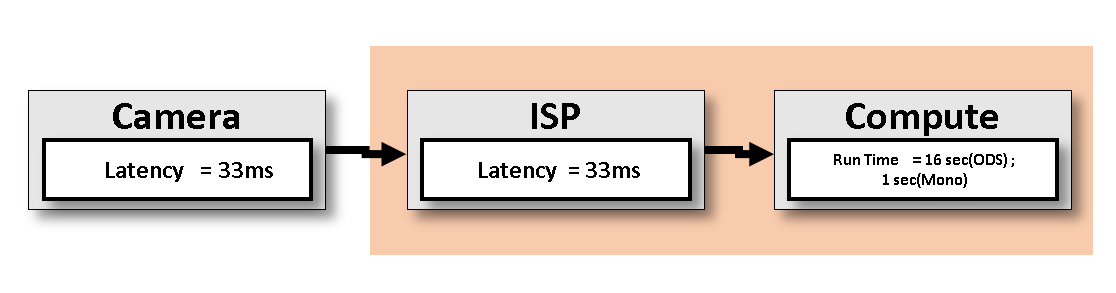
\includegraphics[width=1.1\textwidth]{/media/gunman/Data/thesis/ThesisLatex/data/images/stage_latency.PNG}
		\caption{Latency of Individual Stage}
		\label{fig:ex_4_9}
	\end{center}
	\vspace{-0.3in}
\end{figure} 

We measure the latency of computation in terms of CPU runtime. The optical flow, view synthesis and image sharpening stages take 98\% of total CPU runtime. Of this the major component is optical flow generation which consumes [] percent of runtime. The sharpening stage doesn't seem to benefit the image quality, so we discard the sharpening stage entirely in the current pipeline and leave it for future work. We focus on the optical flow stage which dominates both in terms of memory usage, and computation. 


\subsection{Optical flow runtime breakdown}
Time for each Pyramid search(98\%) as shown in fig 3.1.
\begin{figure}[h]
	\begin{center}
		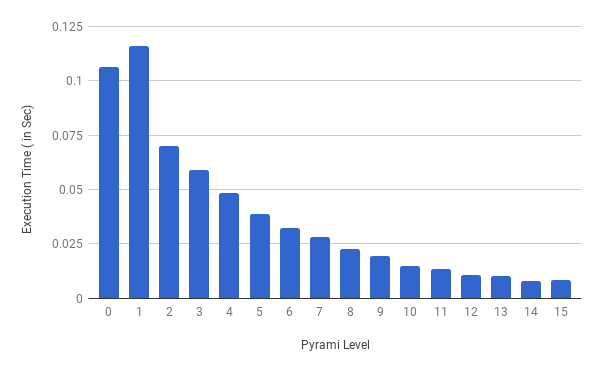
\includegraphics[width=1\textwidth]{/media/gunman/Data/thesis/ThesisLatex/data/images/pyramid_runtime.png}
		\caption{X-axis shows the pyramid level and Y-axis shows the runtime for OF}
		\label{fig:ex_4_9}
	\end{center}
	\vspace{-0.3in}
\end{figure} 

\section{Camera Sensor Configuration}
\subsubsection{Sensor Response Time}
As the ODS consist of several cameras, it makes sense to reconfigure or turn cameras or off based on the application needs and the scene dynamics. If the camera is not moving and certain portions of the camera views are static, the cameras can be reconfigured dynamically to reduce framerate, resolution, or even turn them on and off as per the needs. We observed that the reconfiguration latency is one frame delay if there are no outstanding requests, and if there are pending camera requests, they will be served first before requesting the frame with new configuration. 

The optical flow works well when the image is has high dynamic range. It is possible that some of the regions in the 360 degree view can be in low lightning, while other are in good lightning conditions. In such cases the stitching fails and can have severe artifacts. We can improve the dynamic range of the particular cameras in low lightning by reconfiguring the camera exposure time dynamically. But such approaches doesn't consider the end to end latency of the cameras and camera movements. To account for camera movements, IMU sensor data can be used to make the camera configuration decisions independent of CPU to accelerate the reconfiguration tasks. 

The figures show the differences in low light capture with and without brightness correction.
[Integrate the images with histograms]\newline
	\begin{figure}[h]
	\begin{center}
		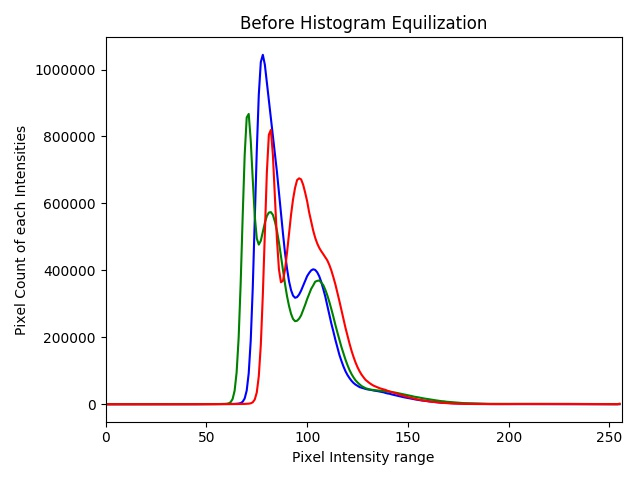
\includegraphics[width=0.7\textwidth]{/media/gunman/Data/thesis/ThesisLatex/data/images/Before_Histogram_equilization.jpg}
		\caption{X-axis shows the pyramid level and Y-axis the runtime tile search and propagate.}
		\label{fig:ex_4_9}
	\end{center}
	\vspace{-0.3in}
\end{figure} 

\begin{figure}[h]
	\begin{center}
		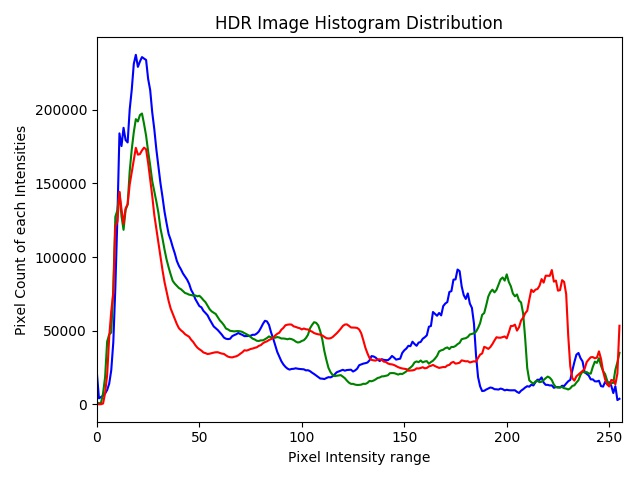
\includegraphics[width=0.7\textwidth]{/media/gunman/Data/thesis/ThesisLatex/data/images/Normal_Histogram_Distribution.jpeg}
		\caption{X-axis shows the pyramid level and Y-axis the runtime tile search and propagate.}
		\label{fig:ex_4_9}
	\end{center}
	\vspace{-0.3in}
\end{figure} 

%On the other hand we observed that when camera is turned on and off, the first few frames are low contrast and less brighter. It takes [3] frames to get the images with good contrast. startup time needs to be less. 
%	Initial frames are low contrast but improves over time. Making case for hardware controller to perform camera configuration. 
	% May be regenerate these figures
	%/media/gunman/Data/Programming/python_coding
%	\begin{figure}[h]
%			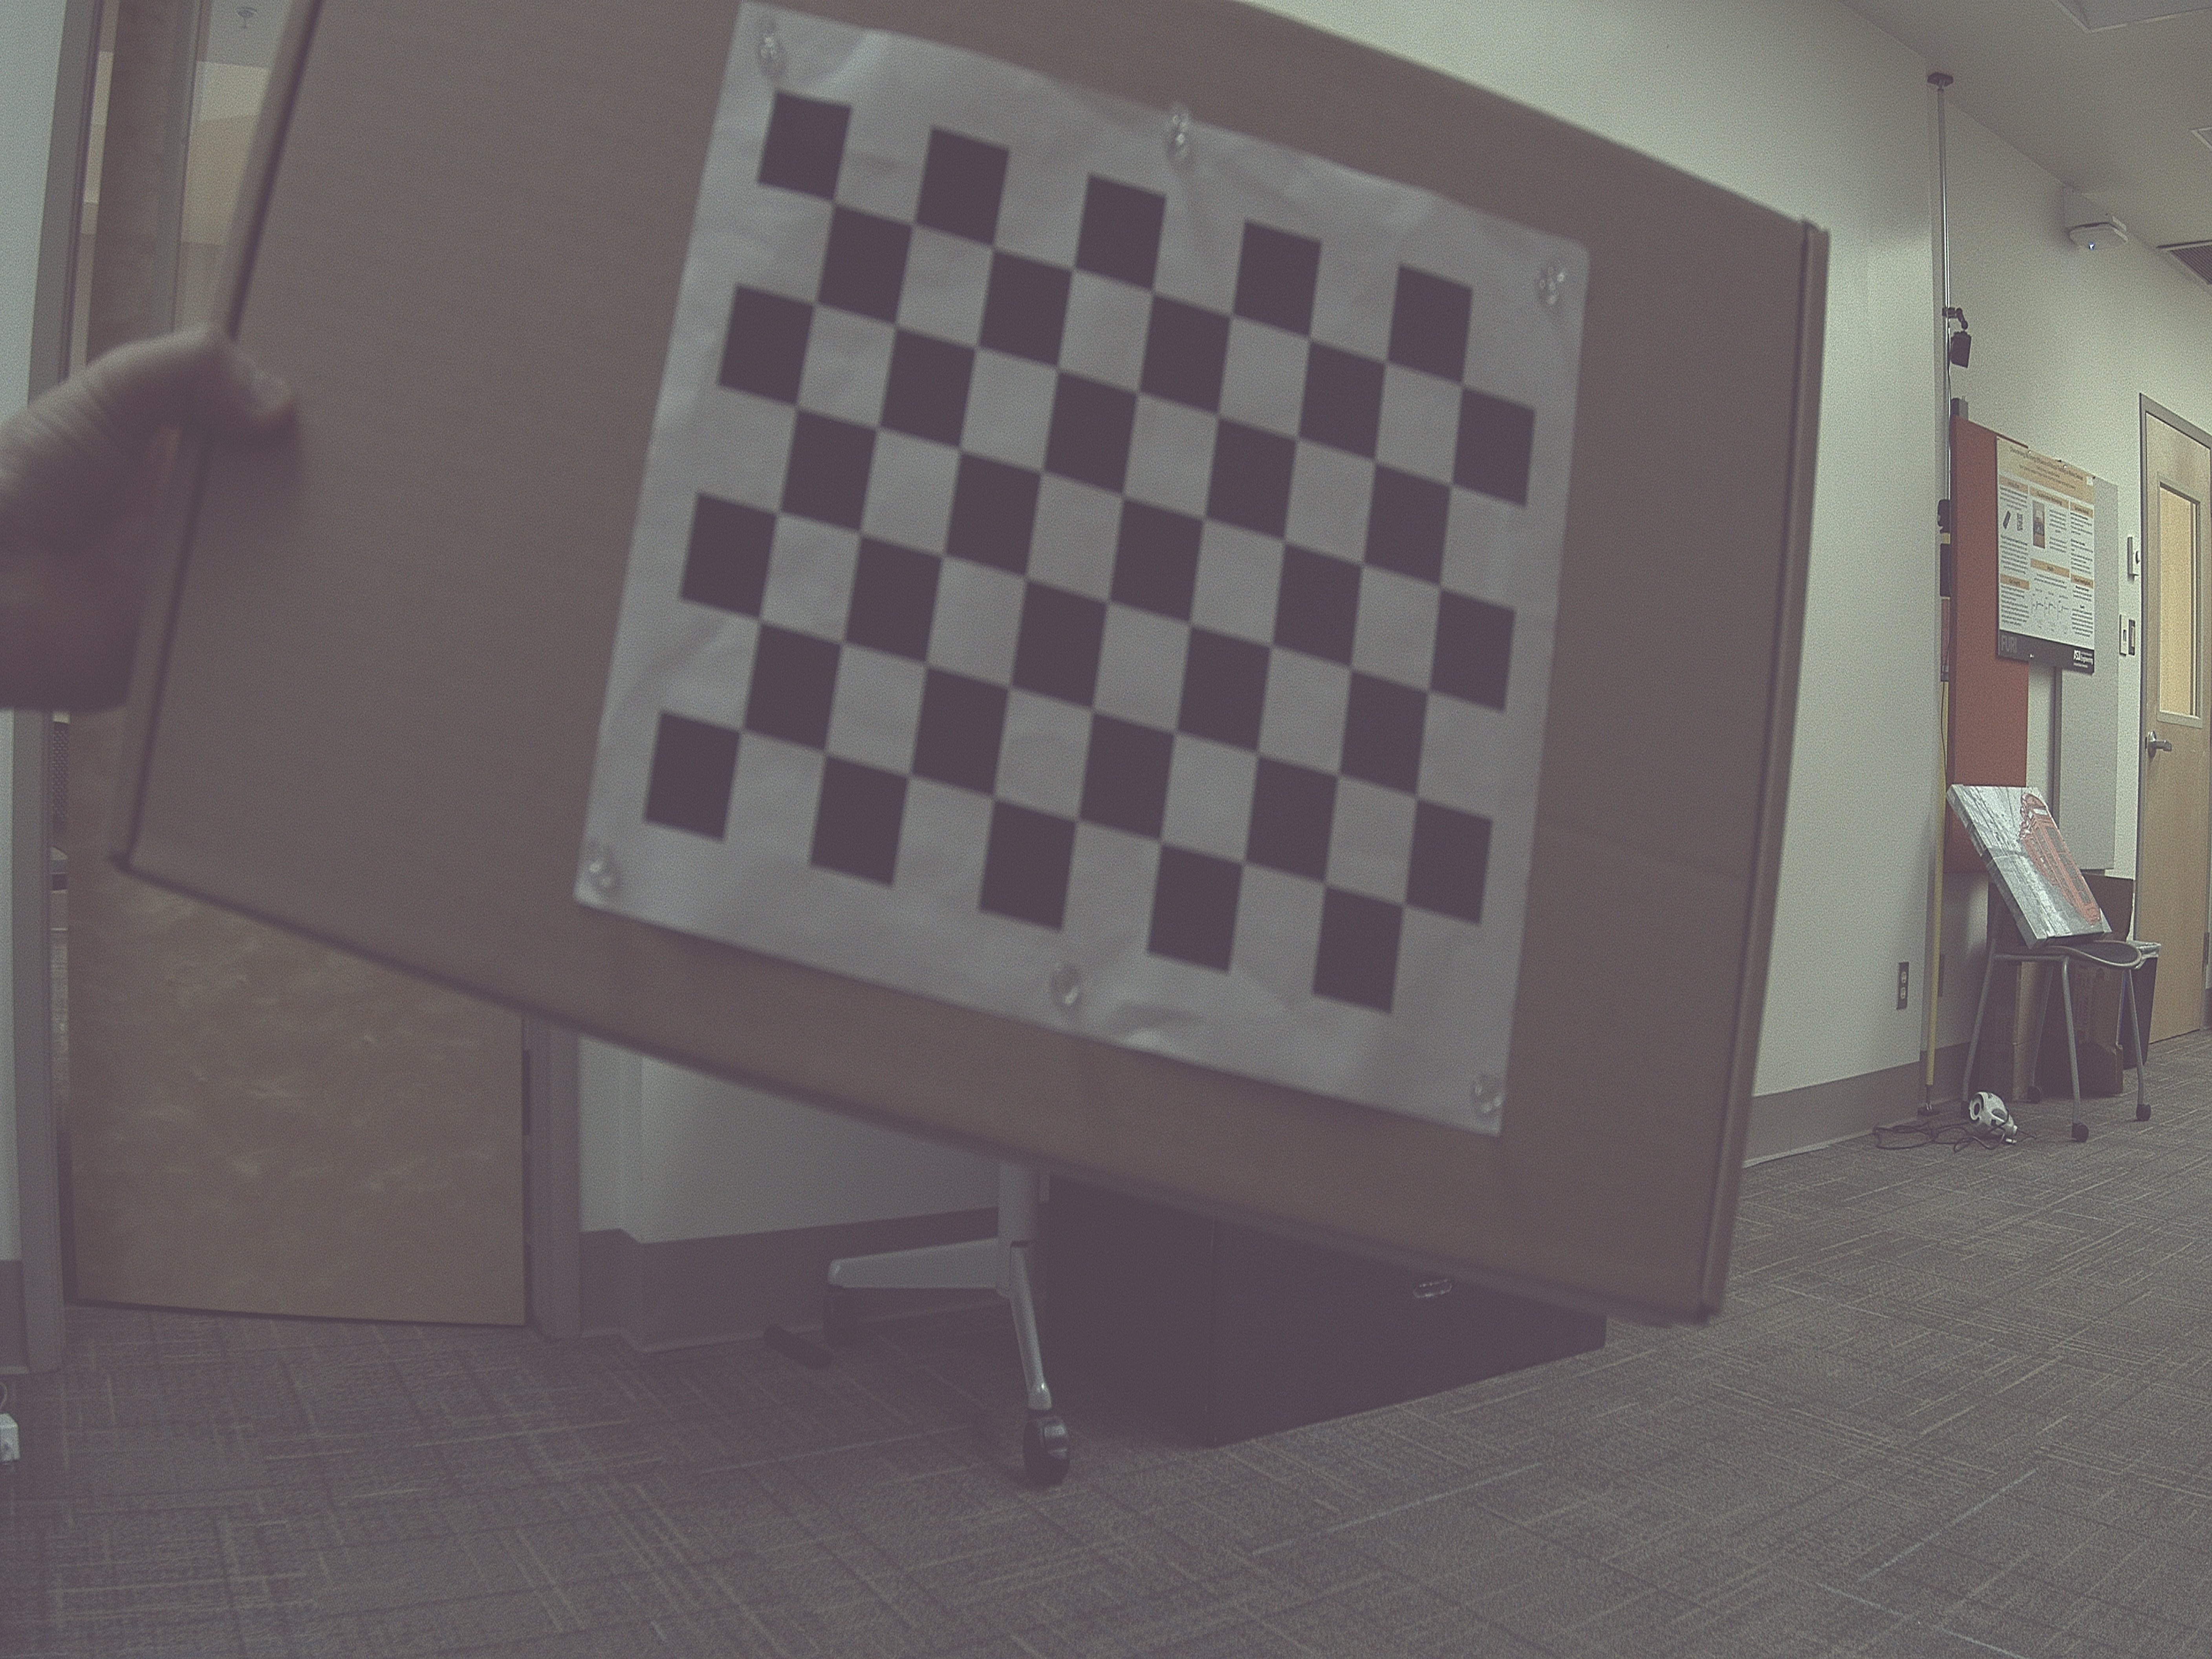
\includegraphics[width=1\textwidth]{/media/gunman/Data/thesis/ThesisLatex/data/images/sensor0_low_contrast.jpg}

\section{Design Scalability}	

\subsubsection{Runtime scalability with the resolution}
As discussed in chapter 2 related work, the resolution required for next generation VR is at-least 16k and frame-rates greater than 120. For our evaluation, we assume that energy scales linear with frame-rate and focus our evaluation on scalability of increasing resolution. We can see in fig that even the runtime scales almost linearly with the resolution. Notice that optical flow dominates the total runtime, followed by view synthesis and image sharpening. We also measure the frequencies of CPU, DRAM controller with increasing resolution and observe [linear] dependency of clock frequency on the resolution.
\begin{figure}[h]
	\begin{center}
		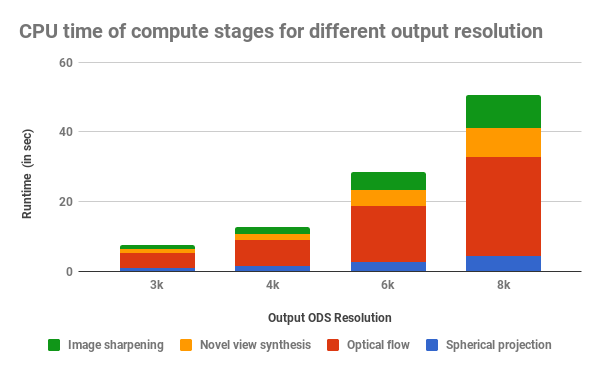
\includegraphics[width=1\textwidth]{/media/gunman/Data/thesis/ThesisLatex/data/images/ExecutionTimeComputeStages.png}
		\caption{CPU execution time of different compute stages. X axis has different sub-stages in optical flow and Y axis correspond to energy per frame.}
		\label{fig:ex_4_9}
	\end{center}
	\vspace{-0.3in}
\end{figure} 

The main takeaway is that the existing hardware and software scale linearly with the increasing resolution and framerate, which is bad considering the VR panorama requirements. We therefore propose directions to exploit the spatio-temporal redundancies within the frame and across the frames to reduce the data flow and computation. We propose rasterbuffer based designs to decrease the chip resources,and using data abstractions at different hardware IP blocks to share data to reduce temporal redundancies(eg. motion vectors from ISP can be used by optical flow stage, thereby removing the necessity to store previous frames and recomputation of motion data at a later time. The same motion vectors can be used to encode spatial frame data to reduce redundant data transfer).
%What is the energy per each output pixel	
%What is energy per pixel when generating only one ODS view, and how does it compare when generating two views! If it is double then we have a problem to solve	
%[Check why sharpening is so costly!]

\subsubsection{Resource scalability with the resolution}
We measure the DRAM capacity required and bandwidth needs as we increase the resolution as a parameter for resource scalability. Higher capacity indicates the need for better encoding schemes and high bandwidth can indicate the temporal redundancy in the data, thereby increasing the bandwidth requirement. For 3k, 4k, 6k and 8k output resolution.

Although we built a system where all the cameras are capturing at same resolution and framerate at a given time, we expect the future cameras make these decisions dynamically to save power. Therefore, we  measure the efficiency of capture and ISP processing at different modes of operation and measure the efficiency of capture and processing in power consumed per pixel at different modes.

%DRAM memory size\newline
%\begin{tabular}{c|c|c|c|c}
%	Stage & 3k & 4k & 6k & 8k \\
%	camera Input & - & - & - & - \\
%	ISP & - & - & - & - \\
%	Motion Estimation & - & - & - & - \\
%	fish2EqRect Projection & - & - & - & - \\
%	Optical Flow & - & - & - & - \\
%	Sharpen & - & - & - & - \\
%\end{tabular} 
%
%\vspace{10mm}
%\begin{tabular}{c|c|c|c|c}
%	o/p Resolution & 3k & 4k & 6k & 8k \\
%	Avg. DRAM BW & - & - & - & - \\
%\end{tabular} 
%\vspace{30mm}

% Figure 
\begin{figure*}
	\begin{center}
		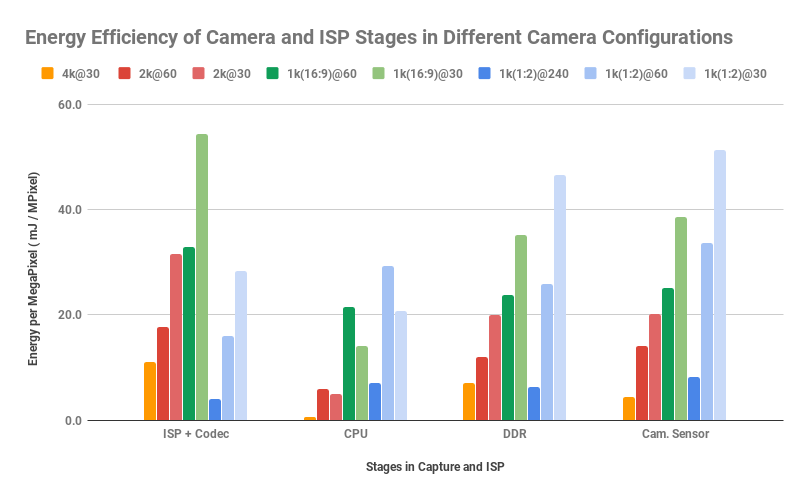
\includegraphics[width=1\textwidth]{/media/gunman/Data/thesis/ThesisLatex/data/images/Power_Efficiency_of_Camera_ISP_Stages_in_different_configurations.png}
		\caption{Power Efficiency of Camera ISP Stages in different configurations}
		\label{fig:ex_4_9}
	\end{center}
	\vspace{-0.3in}
\end{figure*} 

\section{Evaluating data-flow redundancies}
Evaluating redundant computations in optical flow. 
Accuracy Vs Energy\&Perf tradeoff. 
Next we evaluate the optical flow for a scene where foreground has movement and background is static. The temporal flow difference is found out to see the variation of flow. As expected we see the flow change only for the regions where the objects are moving. This observation suggests that accuracy of optical flow can be trade-off with computation time to save energy and latency. It also shows that the accuracy drop is less than \_ percent which can be acceptable


\section{Misc}

	
Increased frame-rate\newline
What is the percentage of new data
ffmpeg I-frame size to the P-frame ratio.
\begin{figure*}
	\begin{center}
		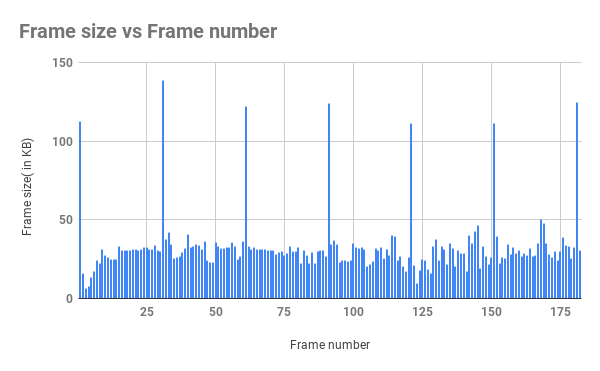
\includegraphics[width=1\textwidth]{/media/gunman/Data/thesis/ThesisLatex/data/images/FramesizevsFramenumber.png}
		\caption{Framesize of I and P frames}
		\label{fig:ex_4_9}
	\end{center}
	\vspace{-0.3in}
\end{figure*} 
%ffprobe lab.mp4 -show_frames
we usually have I,P, and B frames in a compressed video, but in case of realtime compression we will have only I and P frames and disable B frames as it adds latency to the pipeline. Typically I-frame to P-frame is about ~4 times and one I-frame occur for ~30 P-frames. This implies we save a lot on interface power if we can push the computation to near sensor.  
[Numbers - savings from IO datarate reduction]

3) Survey of Camera and ISP stage energy breakdown
Camera Sensor and ISP power directly taken from literature.
Computation Power split into sub stages. \newline
For power characterization of camera sensor and ISP, we run the camera in different resolutions and framerates and see how the various sub-component power changes. The components include Camera Sensor, I/O, ISP, CODEC, DDR, and CPU. The ISP, and CODEC power are combined as they belong to same SOC voltage rail.

The most used configuration for our project when all the six cameras are capturing 1920x1080 @ 30 fps. At this configuration below is the split of different component power. \newline


	e) Quality Tradeoff's with input resolution\newline
Sharpening
Reduction in fidelity of unwarped image, as interpolation is not being done.
Reducing number of pyramid's
f) High motion Vs low motion differences. Size of motion vector to that of size of full frame. 
g) File IO power
h) Breakdown in terms of type of Memory	used
i) Breakdown in terns of type of Computation
j) Breakdown in terms of IO bandwidth bottlenecks
